\section{Introduction}

The baseline design of the CEBAF Large Acceptance Spectrometer for use at the 12~GeV Jefferson Laboratory
(JLab) facility (CLAS12)~\cite{clas12-nim} includes two tracking detector systems. A Silicon Vertex Tracker (SVT)
\cite{svt-nim} consists of a polyhedral arrangement around the target and resides in a 5~T solenoid magnetic field to
detect particles emitted between 40$^\circ$ and 130$^\circ$ with respect to the beam direction. The forward tracking
system consists of drift chambers~\cite{dc-nim} placed before, within, and after a toroidal magnetic field and covers
the polar angle interval between 5$^\circ$ and 35$^\circ$. 

In 2010, a proposal submitted by the IRFU group at CEA-Saclay for an upgrade of the baseline CLAS12 design was
accepted by JLab management. The upgrade of the central tracker consisted of replacing the fourth layer of the SVT
baseline design with 6 layers of cylindrical Micromegas detectors, called the Barrel Micromegas Tracker (BMT). In
addition, a Forward Micromegas Tracker (FMT) made of 6 Micromegas disks was placed $\sim$30~cm downstream of
the target to supplement the forward tracking system with the drift chambers. The FMT and BMT form the Micromegas
Vertex Tracker (MVT). Simulations showed that the addition of the Micromegas detectors improved the vertex and polar
angle resolutions both in the central and in the forward tracking systems compared to the baseline design
\cite{CLAS-NOTE2007-004,CLAS-NOTE2010-003}.

Together, the SVT and the BMT form the Central Vertex Tracker (CVT). The CVT is surrounded by two scintillator-based
detectors called the Central Time-Of-Flight (CTOF)~\cite{ctof-nim} and the Central Neutron Detector (CND)~\cite{cnd-nim}
that provide particle identification information.

\section{System Description}

\subsection{Micromegas Detectors}


\begin{figure*}[!thb]
\begin{center}
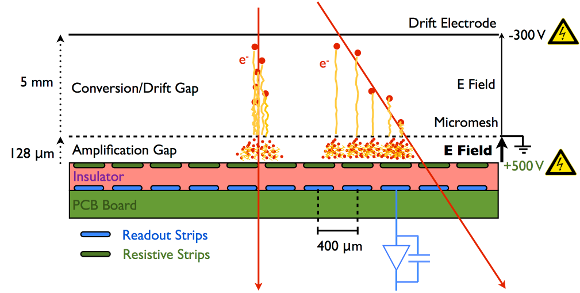
\includegraphics[width=1.8\columnwidth,keepaspectratio]{images/mm_principle}
\end{center}

\caption{Schematic view of a resistive Micromegas detector.}
\label{fig:mm-principle}
\end{figure*}

Micromegas detectors are micro-pattern gaseous detectors \cite{GIOMATARIS199629}. A schematic representation of a
typical Micromegas detector is shown in Fig.~\ref{fig:mm-principle}. In the few-millimeter-wide conversion gap with an
electric field of a few kV/cm, free electrons produced by the ionization of gas molecules by charged particles drift towards
the micro-mesh and enter the amplification gap. In the amplification gap, the electric field reaches several hundreds of
kV/cm, accelerating the electrons arriving from the conversion gap and making them ionize the gas, consequently creating an
electromagnetic shower. The signal is then collected by the readout strips.  


The MVT must sustain a high particle flux, which may induce sparks between the micromesh and the strips in its nominal
running conditions. In order to quench these sparks and their associated temporary high voltages (HV) drops that ``blind''
the detector, all MVT detectors are based on the resistive technology. As depicted in Fig.~\ref{fig:mm-principle}, resistive
strips and a thin layer of insulator are deposited on top of the readout strips \cite{ALEXOPOULOS2011110}. The signals are
transferred from the resistive to the readout strips by capacitive coupling. Finally, the resistive technology allows for higher
gains to be reached compared to regular detectors due to a lower probabilty of sparks in the amplification region. Consequently the resistive technology allows for higher signal to background ratios. In this
configuration the mesh is grounded and the high voltage for amplification is positive on the resistive strips. 

\subsection{General}

The Barrel Micromegas Tracker consists of six layers of cylindrical detectors, three with strips along the beam axis (Z strips)
that provide information about the azimuthal angle of the particle and three with circular strips (C strips) perpendicular to the
beam axis that significantly improves the polar angle determination with respect to that extracted from the SVT information
alone. The strip orientation, the pitch, and the radial distance from the center are listed in 
Table~\ref{tab:bmt_strips}. Each layer is made of three curved detectors covering 115$^\circ$ each. A total of 18 
curved detectors are assembled on a carbon structure to complete the BMT. In addition to the resistive technology, 
these detectors make use of the bulk technology, meaning that the micromesh is embedded with the pillars on top of the 
resistive strips~\cite{GIOMATARIS2006405}. The bulk technology enforces a uniform distance between the micromesh and the 
strips, consequently maintaining a uniform gain over the detector surface, despite the mechanical stress induced by the 
curvature of the tile.

\begin{table}
    \centering
    \begin{tabular}{|c|c|c|}
    \hline
    Radius (mm) & Pitch ($\mu$m) & Strip orientation \\
    \hline
    146.146 & 330 - 860 & C \\
    161.146 & 487 & Z \\
    176.146 & 536 & Z \\
    191.146 & 340 - 770 & C \\
    206.146 & 529 & Z \\
    221.146 & 330 - 670 & C \\
    \hline
    \end{tabular}
    \caption{Radius, pitch, and strip orientation of the different BMT layers.}
    \label{tab:bmt_strips}
\end{table}

\begin{figure}[htb]
 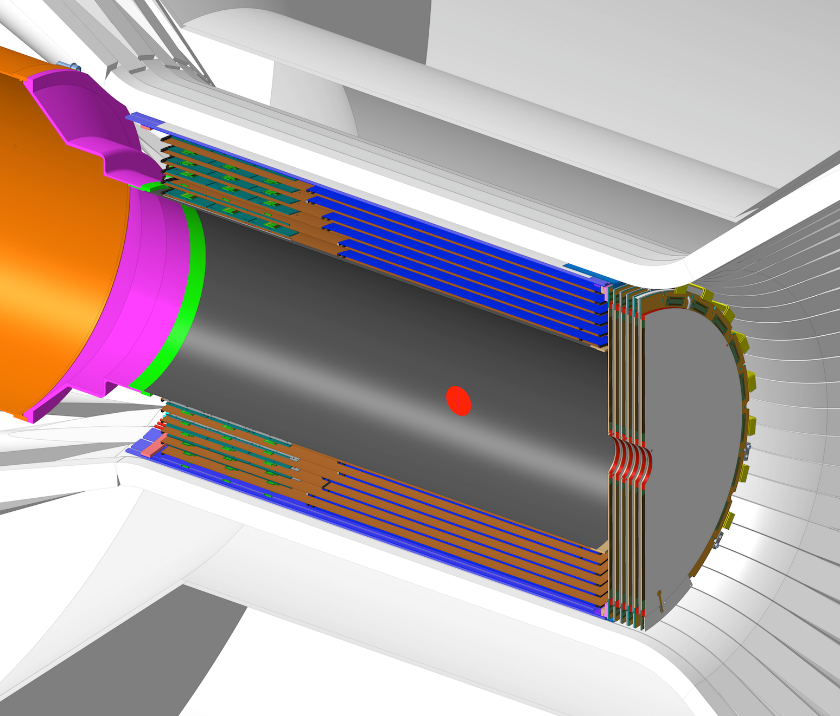
\includegraphics[width=1.0\columnwidth,keepaspectratio]{images/fig1}
 \caption{Cut view showing the 6 different layers of the BMT and the 6 identical FMT disks. The detectors are inserted
   close to the Central Time-of-Flight, itself in the 5~T solenoid magnet. The SVT is inside the MVT and is not displayed in
   this view where the beam enters from the left. The red dot indicates the nominal target position.}
 \label{fig:mm-fig1}
\end{figure}

The Forward Micromegas Tracker consists of six flat Micromegas disks stacked together. The disks are all identical and
assembled with a 60$^\circ$ rotation with respect to one another, giving 3 angles of strips (0$^\circ$, 60$^\circ$, and
120$^\circ$). The FMT is attached to the downstream end flange of the BMT. Figure~\ref{fig:mm-fig1} displays a cut view
of both the BMT and FMT inside the CLAS12 solenoid magnet.

The CLAS12 Forward Tagger (FT) is equipped with four Micromegas disks arranged in two pairs, called the FT
tracker (FT-Trk). The FT-Trk shares most of the design with the FMT and a detailed description can be found in
Ref.~\cite{ft-nim}.

\subsection{Mechanical Structure}

In order to hold the Micromegas Vertex Tracker in the magnet, a stainless-steel tube with the BMT and the FMT at its
downstream end is attached to the flange of the SVT tube structure, as shown in Fig.~\ref{fig:mm-fig2}. This tube also
holds 6 crates containing the 48 readout Front-End Unit (FEU) boards for the Micromegas detectors, as well as the service
distributions for the gas, environmental sensors, and high-voltage distribution. The connection between the detectors and
readout FEUs is done using assembled micro-coaxial cables that allow the signals to be read out from the upstream
electronics crates. Each FEU is connected to a Back-End Unit with an optical fiber. The patch panels for the gas and the high
voltage cables are located on the 6 crates.

\begin{figure}[htb]
 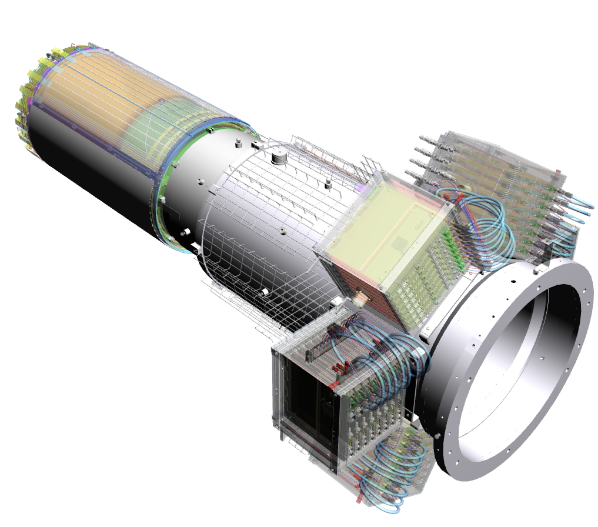
\includegraphics[width=1.0\columnwidth,keepaspectratio]{images/fig2}
 \caption{Support tube with electronics rack and MVT detectors. The beam enters from the right.}
 \label{fig:mm-fig2}
\end{figure}

The mechanical structure of the BMT is made of a thin (1~mm) carbon cylinder with a glued PEEK flange downstream, and a
glued stainless-steel flange upstream, as shown in Fig.~\ref{fig:mm-fig3}. Since the main purpose of the barrel is to
reconstruct protons with momentum as low as 300~MeV, the material budget must be as small as possible in order to reduce
multiple scattering and energy loss. The stainless steel used for the tube and flanges is made of 904L (non-magnetic steel).
The BMT structure is completed by an outer a thin carbon fiber cylinder that protects the BMT tiles during maintenance operations.   
The detector alignment is performed using particle tracks taken during zero magnetic field data taken either with cosmic
rays (as described in Section \ref{sec:cosmics}) or with the electron beam.

\begin{figure}[htb]
 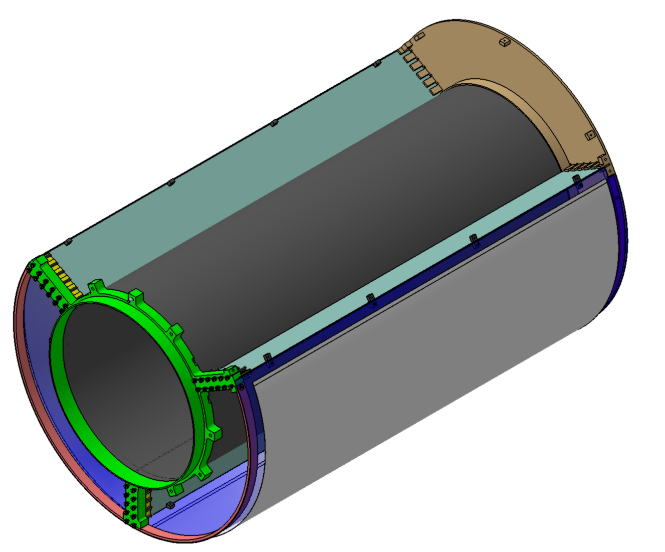
\includegraphics[width=1.0\columnwidth,keepaspectratio]{images/fig3}
 \caption{BMT mechanical structure shown with one sector open that houses 6 curved detectors.}
 \label{fig:mm-fig3}
\end{figure}

\subsection{Barrel Micromegas Tracker (BMT)}

The Barrel detector tiles are made of a thin printed circuit board (PCB) (0.2~mm) transformed into Micromegas with the bulk
process. Up to 16 MEC8 connectors are welded on the upstream end of the tile. The PCB is curved on a custom mandrel tool
with the desired radius. The cylindrical shape is then maintained by gluing two carbon fiber arcs at each end of the active
zone and two aluminum arcs on the MEC8 connector side. The thickness of the carbon and aluminum structure arcs (3~mm)
was chosen to match the design drift gap of the detectors. A Kapton foil (0.25~mm) with metallic coating is then glued on top
of the carbon-aluminum structure to seal the detector and serves as the drift electrode of the detector. A curved 3D-printed
plastic mechanical bracket is attached above the connectors to provide rigidity for the connection of the signal cables. The high
voltage connections and the associated protection circuit are hosted inside 4~cm $\times$ 8~cm metallic boxes on the upstream side of
the PCB, out of the active area.  Gas is introduced in the middle of the connector side and flushed out on the edges of the connector side through the
hollow carbon-aluminum mechanical structure. The leak rate of each detector is measured below \(2\times10^{-3}\)~l/hr. Pins,
serving both as fixation points and for alignment, are inserted and glued on both ends of each carbon tube. A geometrical survey
was performed and the measured radii are within 1 to 2~mm of the design values. Figure~\ref{fig:mm-fig4} shows a view of the
curved BMT detectors.

\begin{figure}[htb]
 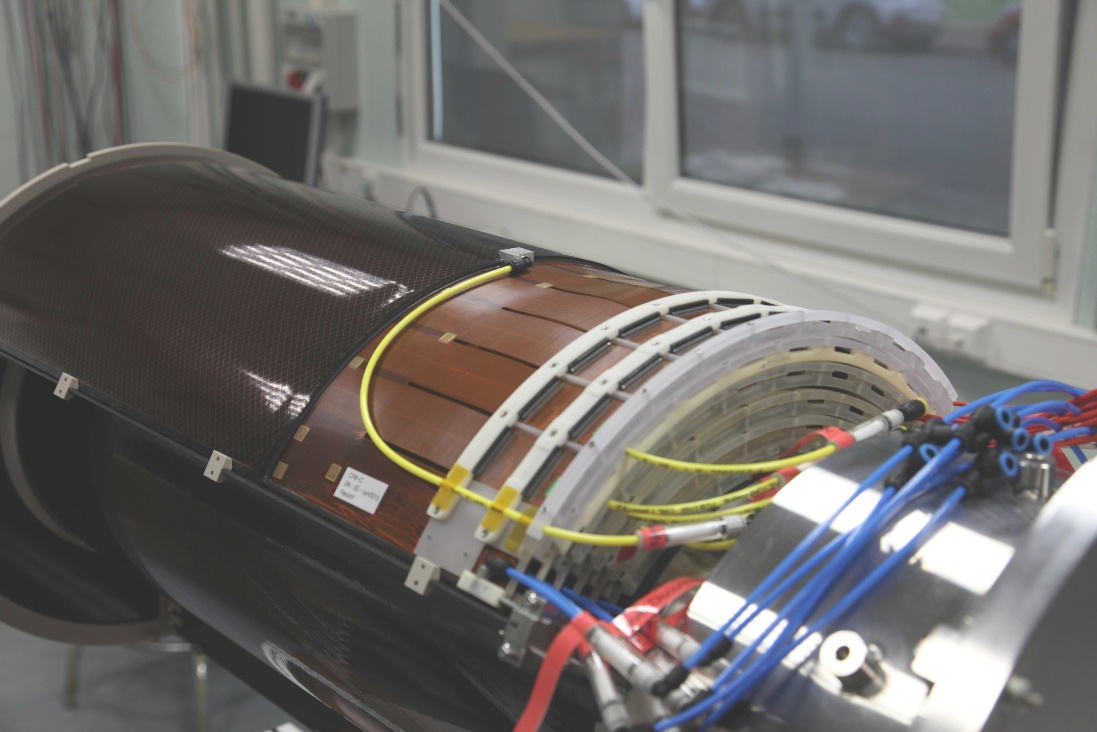
\includegraphics[width=1.0\columnwidth,keepaspectratio]{images/fig5}
 \caption{Photograph of a full stack of 6 BMT layers. The two aluminum arcs are visible on top of the connectors. The blue and
   yellow plastic tubes are part of the gas plumbing.}
 \label{fig:mm-fig4}
\end{figure}

As pointed out above, the BMT is located inside the 5~T solenoid. The high magnetic field had a strong impact on the design and
operation of the BMT detectors. Since the (detector) electric and the (solenoid) magnetic fields are essentially orthogonal, the
primary electrons in the drift region of the Micromegas detectors are subject to Lorentz forces. Consequently, the electron
trajectories form an angle with respect to the electric field direction, the so-called Lorentz angle. Hence, the charge is spread
over a large area and this directly impacts the position resolution. Early studies showed that large Lorentz effects could be
partly compensated for by using a 5-6~kV/cm drift high voltage~\cite{KONCZYKOWSKI2010274}. This increase of the drift
field impacts the efficiency through a loss of transparency of about \(\approx5\%\). The effect is worse in the case of the
Z-type detectors with their strips parallel to the B-field direction. Finally, the gas mixture of 90\% argon + 10\% isobutane
offers a reasonable trade-off between a limited drift velocity to reduce the Lorentz force effects and a high number of
electrons generated in the conversion gap. The Lorentz angle is estimated to be about 40$^\circ$ at 5kV/cm drift electric field at 5 Tesla magnetic field.

\subsection{Forward Micromegas Tracker (FMT)}

The Forward Micromegas Tracker, shown in Fig.~\ref{fig:mm-fig5}, consists of six identical Micromegas resistive detectors in
the forward region from 30~cm to 36~cm downstream of the target center. Each Micromegas detector is a 450~mm diameter disk with an
active area of 1024 parallel readout strips (525~$\mu$m pitch). The angle between the strip orientation of two adjacent disks
is 60$^\circ$. The distance between the readout strips of two consecutive disks is 10.5~mm.  Each disk consists of an assembly
of two 0.2~mm thick PCBs glued on a 2~mm Rohacell foam backing to form the readout plane and a 0.2~mm PCB for the drift plane
glued on two cylindrical frames that define the gas volume (5~mm). The inner frame is made of PEEK and the outer frame of
aluminum. Both define the chamber and are attached to the readout plane using stainless steel screws. High voltage connections
and associated filter circuits are located on the disk edge diametrically opposed from one another. The signals are read out via
16 MEC8 connectors.

\begin{figure*}[htb]
 
 \begin{center}
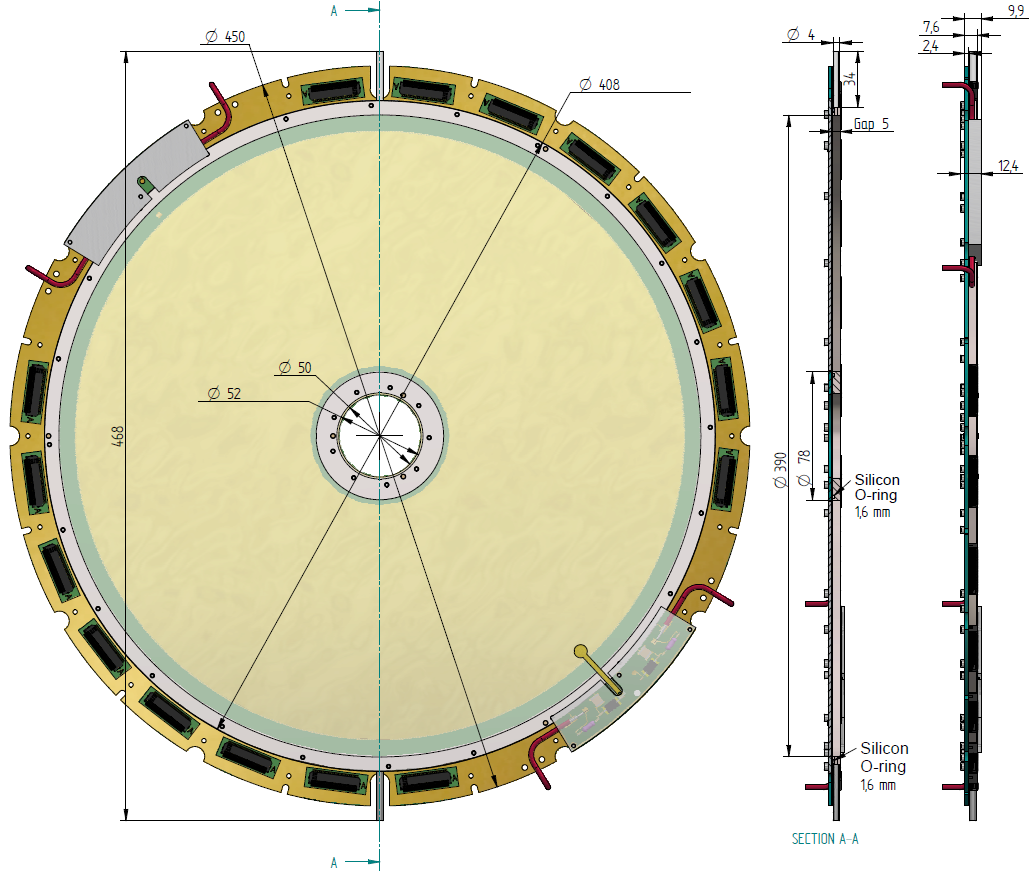
\includegraphics[width=1.2\columnwidth,keepaspectratio]{images/fig6_1}
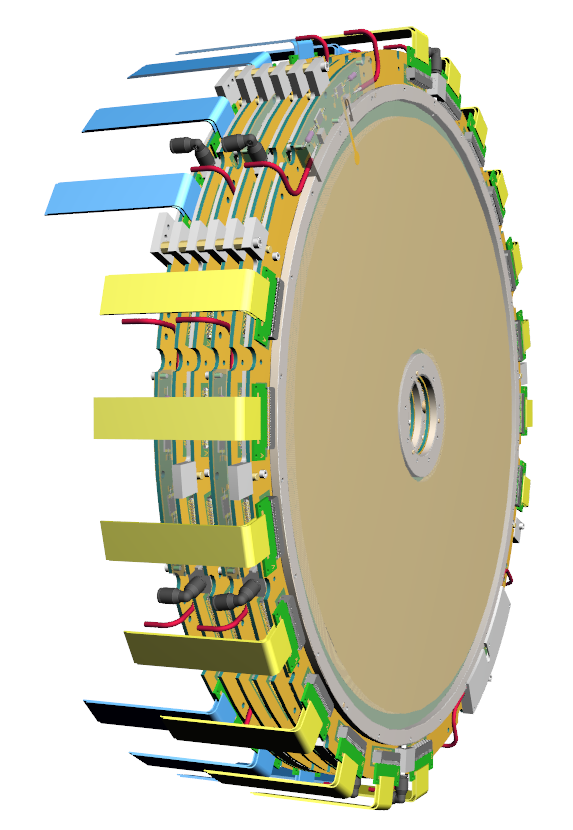
\includegraphics[width=0.6\columnwidth,keepaspectratio]{images/fig6_2}
 \end{center}
 
 \caption{CAD views of the FMT disks.}
 \label{fig:mm-fig5}
\end{figure*}

The active area of the FMT is divided in two parts, the inner part with diameter $86 < d < 166$~mm, and the outer part with
$168 < d < 380$~mm. Each of the two parts can be independently energized so that the inner region can be turned off in the
case of a very high flux of charged particles.

Since the magnetic field is parallel to the drift field in the FMT, the drift electrons are not affected by the Lorentz angle
effect. In order to improve timing resolution, a mixture of 80\% argon + 10\% isobutane + 10\% CF$_4$ allows for an increase
of the drift velocity compared to 90\% argon + 10\% isobutane mixture used in the BMT~\cite{GAS}. 

\subsection{Gas System}

The Micromegas are continuously flushed with gas in order to maintain high purity and to overcome the normal outgassing of the
detectors. As stated above, the gas used for the BMT is a flammable mixture, argon with 10\% isobutane. Each layer of the
barrel is fed with one gas line. The tiles of a given layer are connected in series, with a flow rate of about 1.5~l/hr. For the FMT,
the gas mixture is argon with 10\% CF$_4$ and 10\% isobutane with a flow rate of 2~l/hr for a set of three disks connected
in series. Thus a total of $\sim$13~l/hr is used for both the FMT and BMT. Due to the low gas flow rate for the detectors, a gas
recirculation system is not employed for the MVT. 

\begin{figure*}[htb]
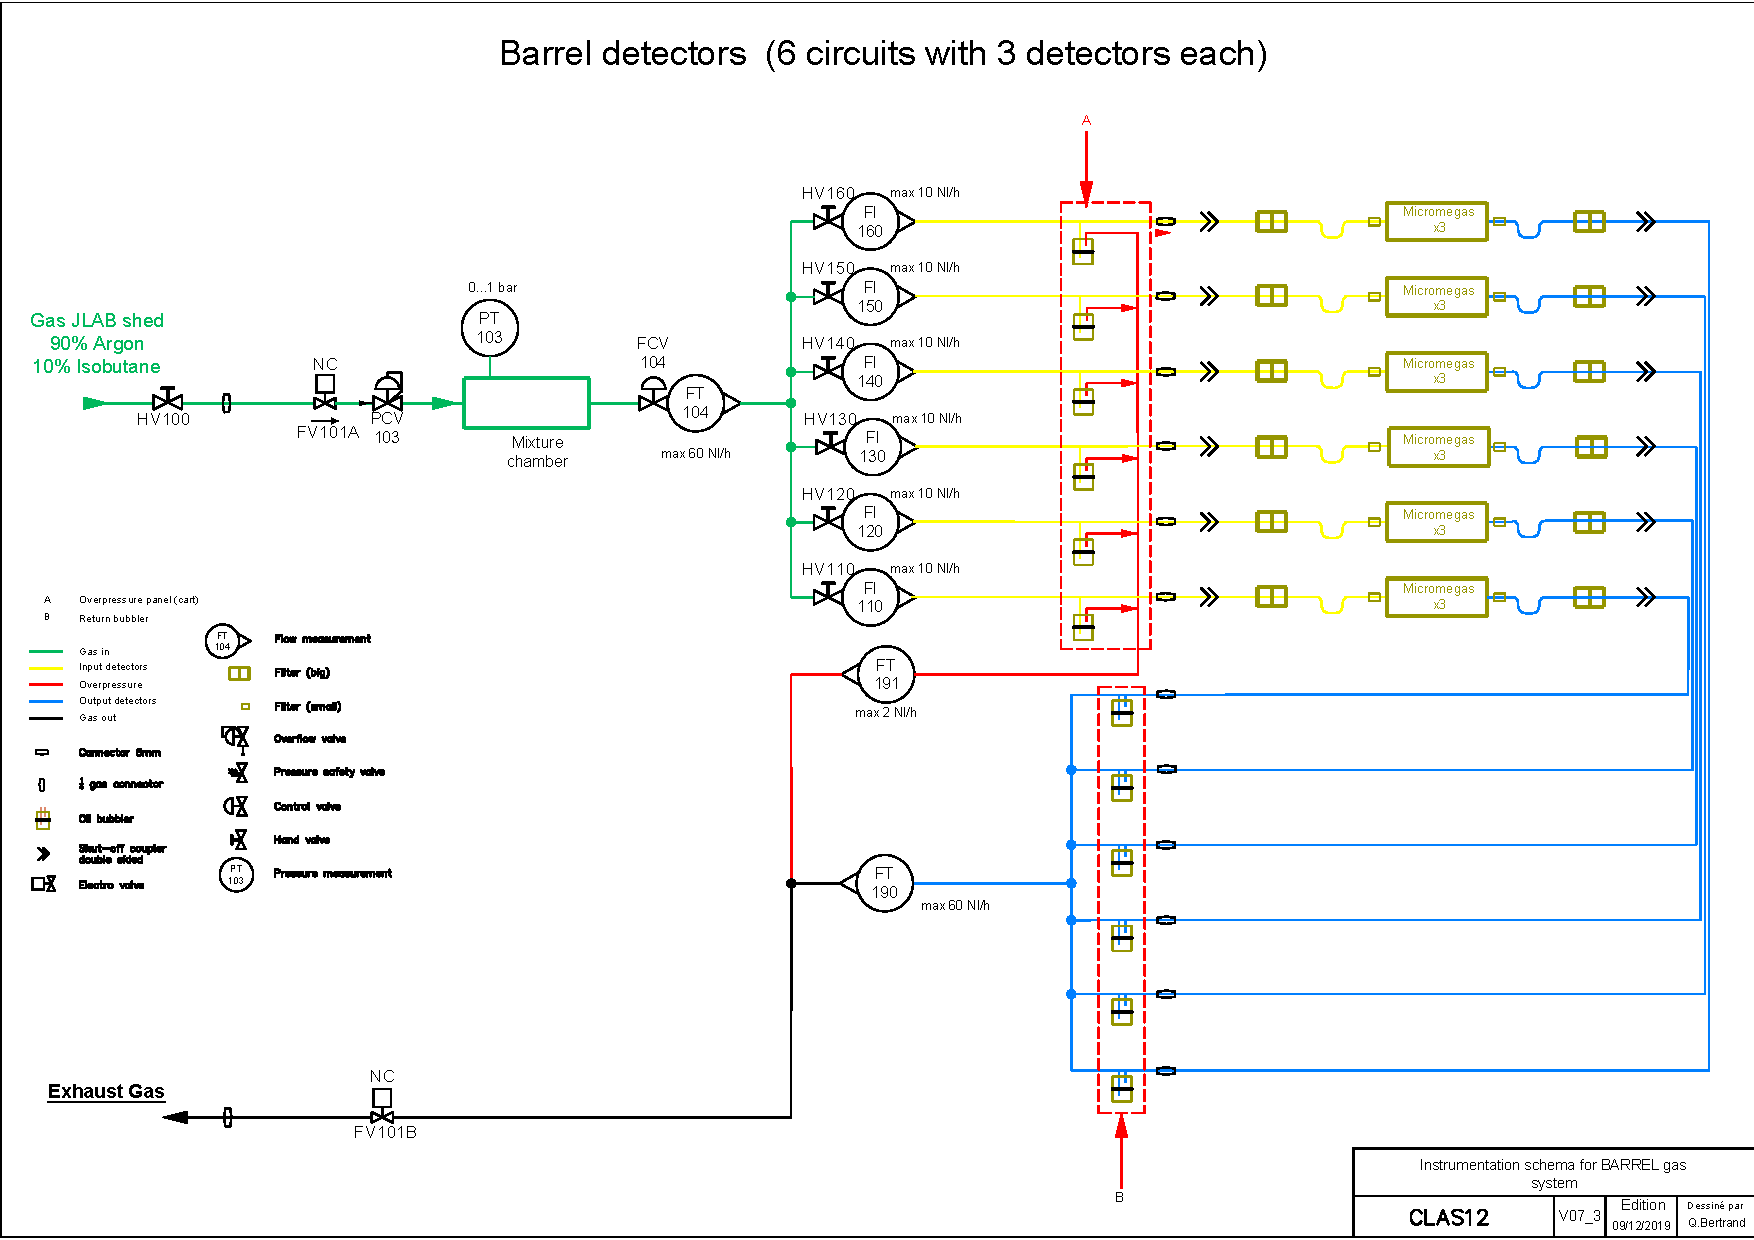
\includegraphics[width=2\columnwidth,keepaspectratio]{images/Clas12_Barrel_V07_2}
 \caption{Gas distribution diagram for the Barrel Micromegas Tracker.}
 \label{fig:mm-gas-sys-barrel}
\end{figure*}


\begin{figure*}[htb]
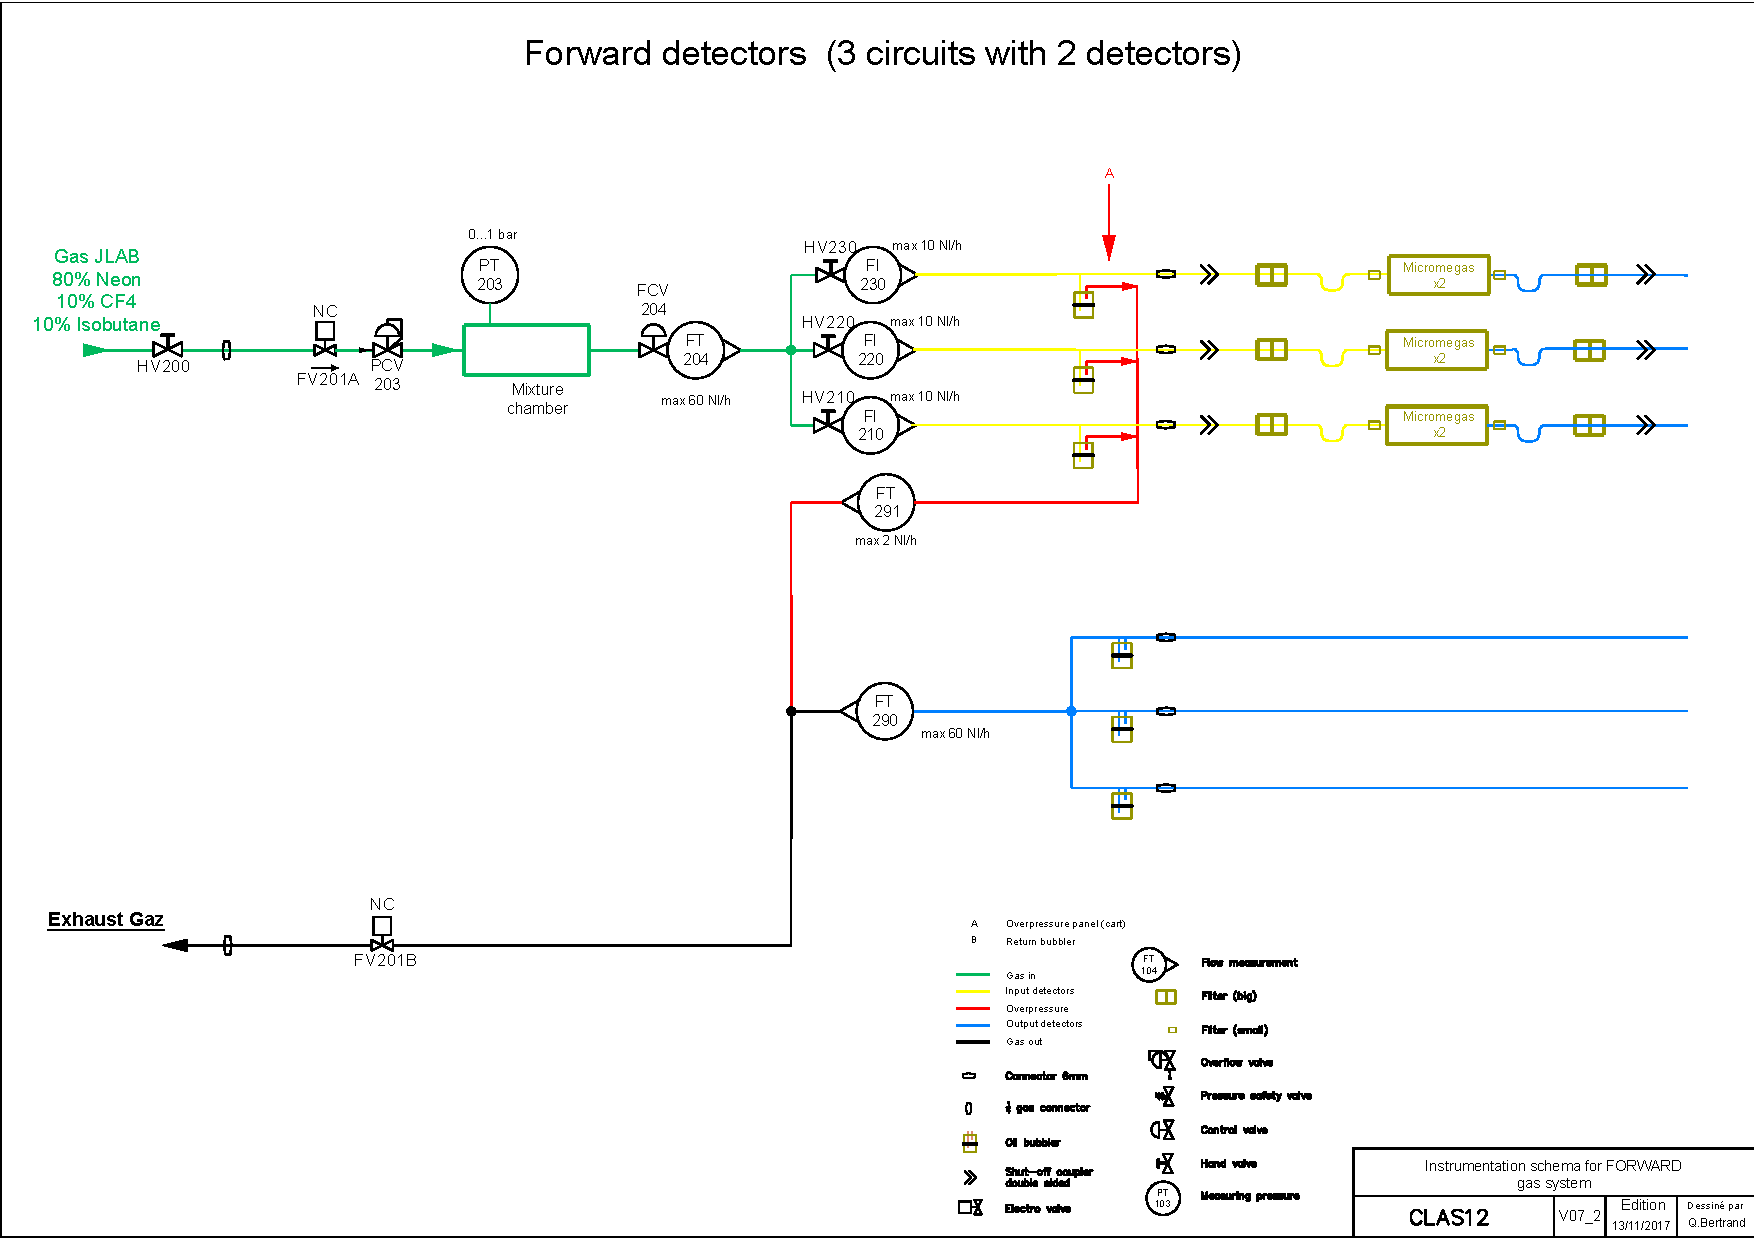
\includegraphics[width=2\columnwidth,keepaspectratio]{images/Clas12_Forward_V07_2}
 \caption{Gas distribution diagram for the Forward Micromegas Tracker.}
 \label{fig:mm-gas-sys-forward}
\end{figure*}

A programmable logic controller controls the overall flow sent to the BMT and to the FMT, which is provided by a gas mixing
system located outside of the experimental hall. As shown in Fig.~\ref{fig:mm-gas-sys-barrel} and 
Fig.~\ref{fig:mm-gas-sys-forward}, a gas control panel allows the gas
distribution between the different lines for the BMT and FMT to be manually adjusted . Inside the gas control panel, the gas
pressure and flow are measured at various points. The flow rate and pressure must be low and controlled to avoid any
deformation of the detectors. Interlocks are set to close valves and stop the gas flow in the detector if pressures or flows are
above the set thresholds. Finally, the total inflow and outflow are compared and trigger an interlock to stop the gas flow if they
disagree, which could indicate a leak in the gas system or the detector volume. 
